\chapter{Chemical Aspects of Life}\label{chemical-aspects-of-life}

\href{https://en.wikipedia.org/wiki/Matter}{Everything that we can bump
into, touch or squeeze including living things are composed of atoms.}
\href{https://en.wikipedia.org/wiki/Chemical_element}{Chemical elements}
are pure substances of one type of
\href{https://en.wikipedia.org/wiki/Atom}{atom}. Atoms combine to form
\href{https://en.wikipedia.org/wiki/Molecule}{molecules}. Molecules
combined of more than one element are called compounds.

Commonly people distinguish between organic and inorganic compounds.
However, there is no clear or universally agreed-upon distinction
between organic and inorganic compounds. Organic chemists traditionally
and generally refer to any molecule containing carbon as an organic
compound and by default this means that inorganic chemistry deals with
molecules lacking carbon. As many minerals are of biological origin,
biologists may distinguish organic from inorganic compounds in a
different way that does not hinge on the presence of a carbon atom.
Pools of organic matter, for example, that have been metabolically
incorporated into living tissues persist in decomposing tissues, but as
molecules become oxidized into the open environment, such as atmospheric
CO\textsubscript{2}, this creates a separate pool of inorganic
compounds. The International Union of Pure and Applied Chemistry
(IUPAC), an agency widely recognized for defining chemical terms, does
not offer definitions of inorganic or organic compounds. Hence, the
definition for an inorganic versus an organic compound in a
multidisciplinary context spans the division between organic life living
(or animate) and inorganic non-living (or inanimate) matter. In broader
speech, the term commonly referred to compounds synthesized by purely
geological systems, in contrast to those with a biological component in
their origin.

Cells consist mostly of water (70\%-90\%). The bulk of their dry weight
consists of compounds containing the elements carbon (C), hydrogen (H),
oxygen (O), nitrogen (N), and phosphorus (P). The four major types of
organic biomolecules are carbohydrates, lipids, proteins and nucleic
acids. The more complex members of these categories (biomacromolecules)
are made up of chains of smaller molecules (monomers) strung together
more or less like beads in a necklace. These complex molecules are
called polymers. In living organisms, polymers are made by dehydration
synthesis, the loss of a water molecule between each pair of monomers.
Conversely, polymers can be digested (broken up into monomers) by the
addition of a molecule of water between each pair of monomers. This
process is known as hydrolysis.

Carbohydrates are biomolecules consisting of carbon (C), hydrogen (H)
and oxygen (O) atoms, usually with a hydrogen to oxygen atom ratio of
2:1 (as in water) with the formula
C\textsubscript{n}(H\textsubscript{2}O)\textsubscript{n}.

Lipids are substances of biological origin that are insoluble in water.
Lipids comprise a group of naturally occurring molecules that include
fats, waxes, sterols, fat-soluble vitamins (such as vitamins A, D, E,
and K), monoglycerides, diglycerides, triglycerides, and phospholipids.
The main biological functions of lipids include storing energy,
signaling, and acting as structural components of cell membranes.

Proteins are large biomolecules consisting of one or more long chains of
amino acids linked by peptide bonds. Proteins perform a vast array of
functions within organisms, including catalyzing metabolic reactions,
DNA replication, responding to stimuli, and transporting molecules from
one location to another. Proteins differ from one another primarily in
their sequence of amino acids, which is dictated by the nucleotide
sequence of their genes, and which usually results in protein folding
into a specific three-dimensional structure that determines its
activity.

\begin{figure}

{\centering 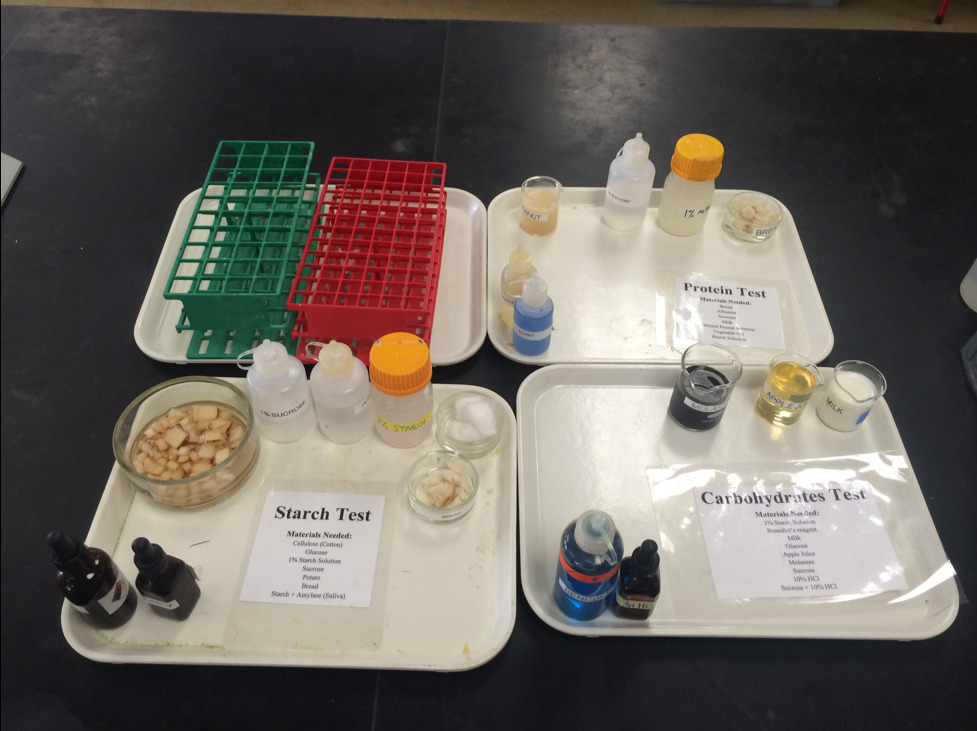
\includegraphics[width=0.7\linewidth]{./figures/chem_aspects/Setup}

}

\caption{Experimental materials for this lab}\label{fig:setup}
\end{figure}

\section{Test for Reducing sugars}\label{test-for-reducing-sugars}

A \href{https://en.wikipedia.org/wiki/Reducing_sugar}{reducing sugar} is
one that reduces another compound and is itself oxidized; that is, the
carbonyl carbon of the sugar is oxidized to a carboxyl group. A reducing
sugar has a free aldehyde group or a free ketone group. All
monosaccharides are reducing sugars, along with some disaccharides,
oligosaccharides, and polysaccharides. Monosaccharides which contain an
aldehyde group are known as aldoses, and those with a ketone group are
known as ketoses. The aldehyde can be oxidized via a redox reaction in
which another compound is reduced. Thus, a reducing sugar is one that
reduces certain chemicals. Sugars with ketone groups in their open chain
form are capable of isomerizing via a series of tautomeric shifts to
produce an aldehyde group in solution. Therefore, ketone-bearing sugars
like fructose are considered reducing sugars but it is the isomer
containing an aldehyde group which is reducing since ketones cannot be
oxidized without decomposition of the sugar. This type of isomerization
is catalyzed by the base present in solutions which test for the
presence of aldehydes. Aldoses or aldehyde-bearing sugars are reducing
also because during oxidation of aldoses, there are certain oxidizing
agents that are reduced. The common dietary monosaccharides galactose,
glucose and fructose are all reducing sugars. Many disaccharides, like
lactose and maltose, also have a reducing form, as one of the two units
may have an open-chain form with an aldehyde group. However, sucrose is
a non-reducing disaccharide since neither of the rings is capable of
opening. Benedict's reagent (Cu\textsuperscript{2+} in aqueous sodium
citrate) is used as a qualitative test to detect the presence of
reducing sugars. The reducing sugar reduces the copper(II) ions to
copper(I), which then forms a brick red copper(I) oxide precipitate.

\begin{figure}

{\centering 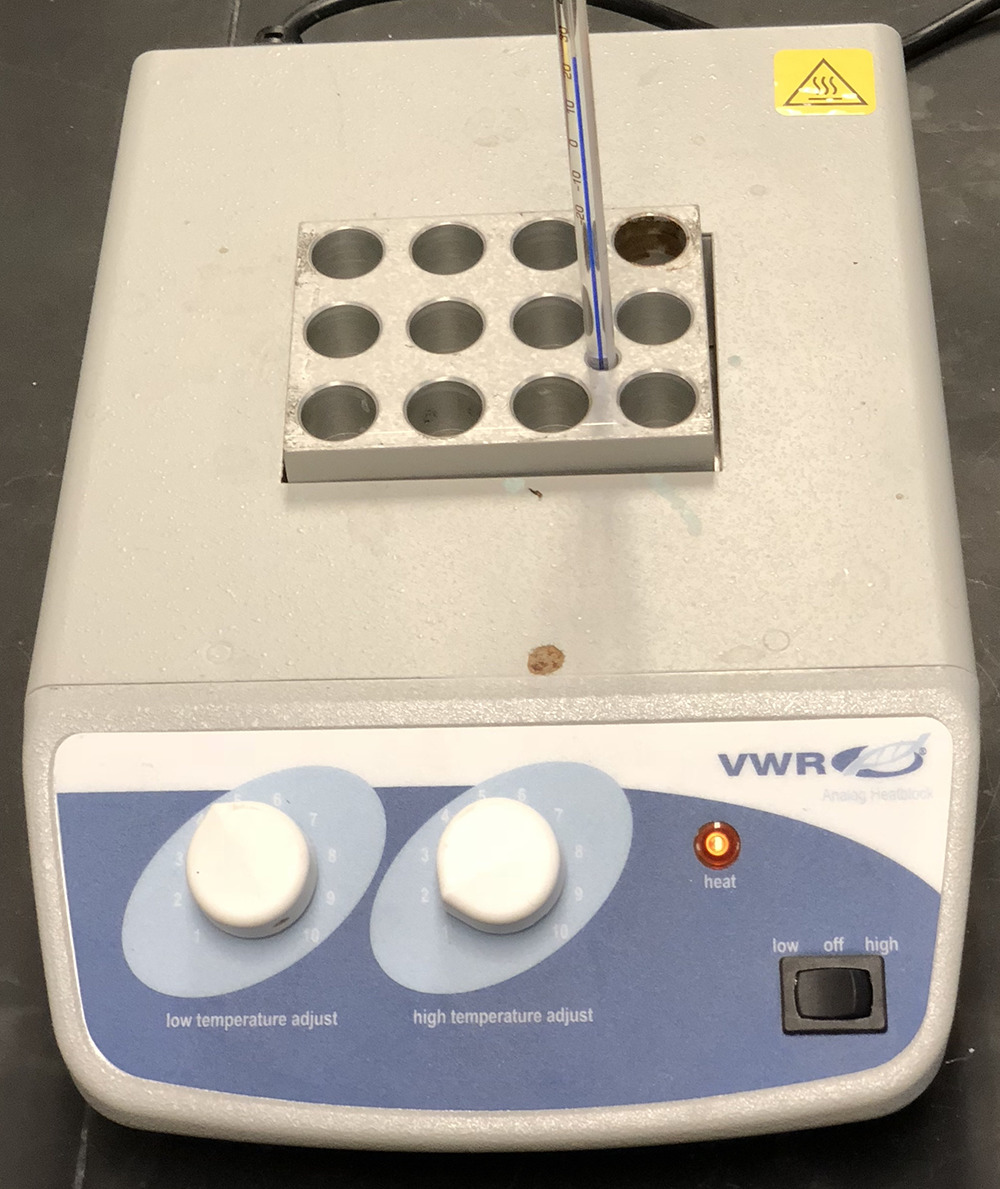
\includegraphics[width=0.7\linewidth]{./figures/chem_aspects/Heatblock}

}

\caption{Heat block ("dry bath")}\label{fig:heatblock}
\end{figure}

\subsection{Experimental procedures}\label{experimental-procedures-1}

\begin{enumerate}
\def\labelenumi{\arabic{enumi}.}
\tightlist
\item
  Turn on the 65°C heat block (Figure \ref{fig:heatblock}) by pushing
  the little black switch on the lower right side of the to ``high''.
  Rotate the white ``high temperature adjust'' button to number 3.
\item
  Turn on the 37°C heat block by pushing the little black switch on the
  lower right side of the to ``low''. Rotate the white ``low temperature
  adjust'' button to number 4.
\item
  Obtain 7 plastic test tubes and a test tube rack.
\item
  Using a wax pencil,label each tube with a number (1 to 7).
\item
  Place the tubes from left (tube \#1) to right (tube \#7) in the first
  row of a test tube rack.
\item
  Add the test material each tube as indicated in Table \ref{tab:sugar}.
\item
  Add 2 ml of Benedict's reagent to each tube using a plastic transfer
  pipette. Figure 5 Plastic transfer pipette (3 ml capacity.
\item
  Mix well.
\item
  Check the that the temperature of the heat block is
  \textasciitilde{}65°C and then place the tubes in the heat block. Set
  a timer and incubate the tubes for 15 minutes. Begin setting up
  Experiment 2 (below) while the tubes are incubating.
\item
  After 15 minutes, remove the tubes using a test tube holder (be
  careful, they are hot!), place them in the tube rack and record the
  color (in your own words) in Table \ref{tab:sugar}.
\end{enumerate}

\begin{longtable}[]{@{}clccc@{}}
\caption{\label{tab:sugar} Test for reducing sugars.}\tabularnewline
\toprule
Tube \# & Test material & Benedict's & Observed color & Test Result (+
or -)\tabularnewline
\midrule
\endfirsthead
\toprule
Tube \# & Test material & Benedict's & Observed color & Test Result (+
or -)\tabularnewline
\midrule
\endhead
1 & 2 ml H\textsubscript{2}O & 2 ml & &\tabularnewline
2 & 2 ml glucose & 2 ml & &\tabularnewline
3 & 2 ml milk & 2 ml & &\tabularnewline
4 & 2 ml apple juice & 2 ml & &\tabularnewline
5 & 2 ml starch & 2 ml & &\tabularnewline
6 & 2 ml molasses & 2 ml & &\tabularnewline
7 & 2 ml sucrose & 2 ml & &\tabularnewline
\bottomrule
\end{longtable}

\begin{figure}

{\centering 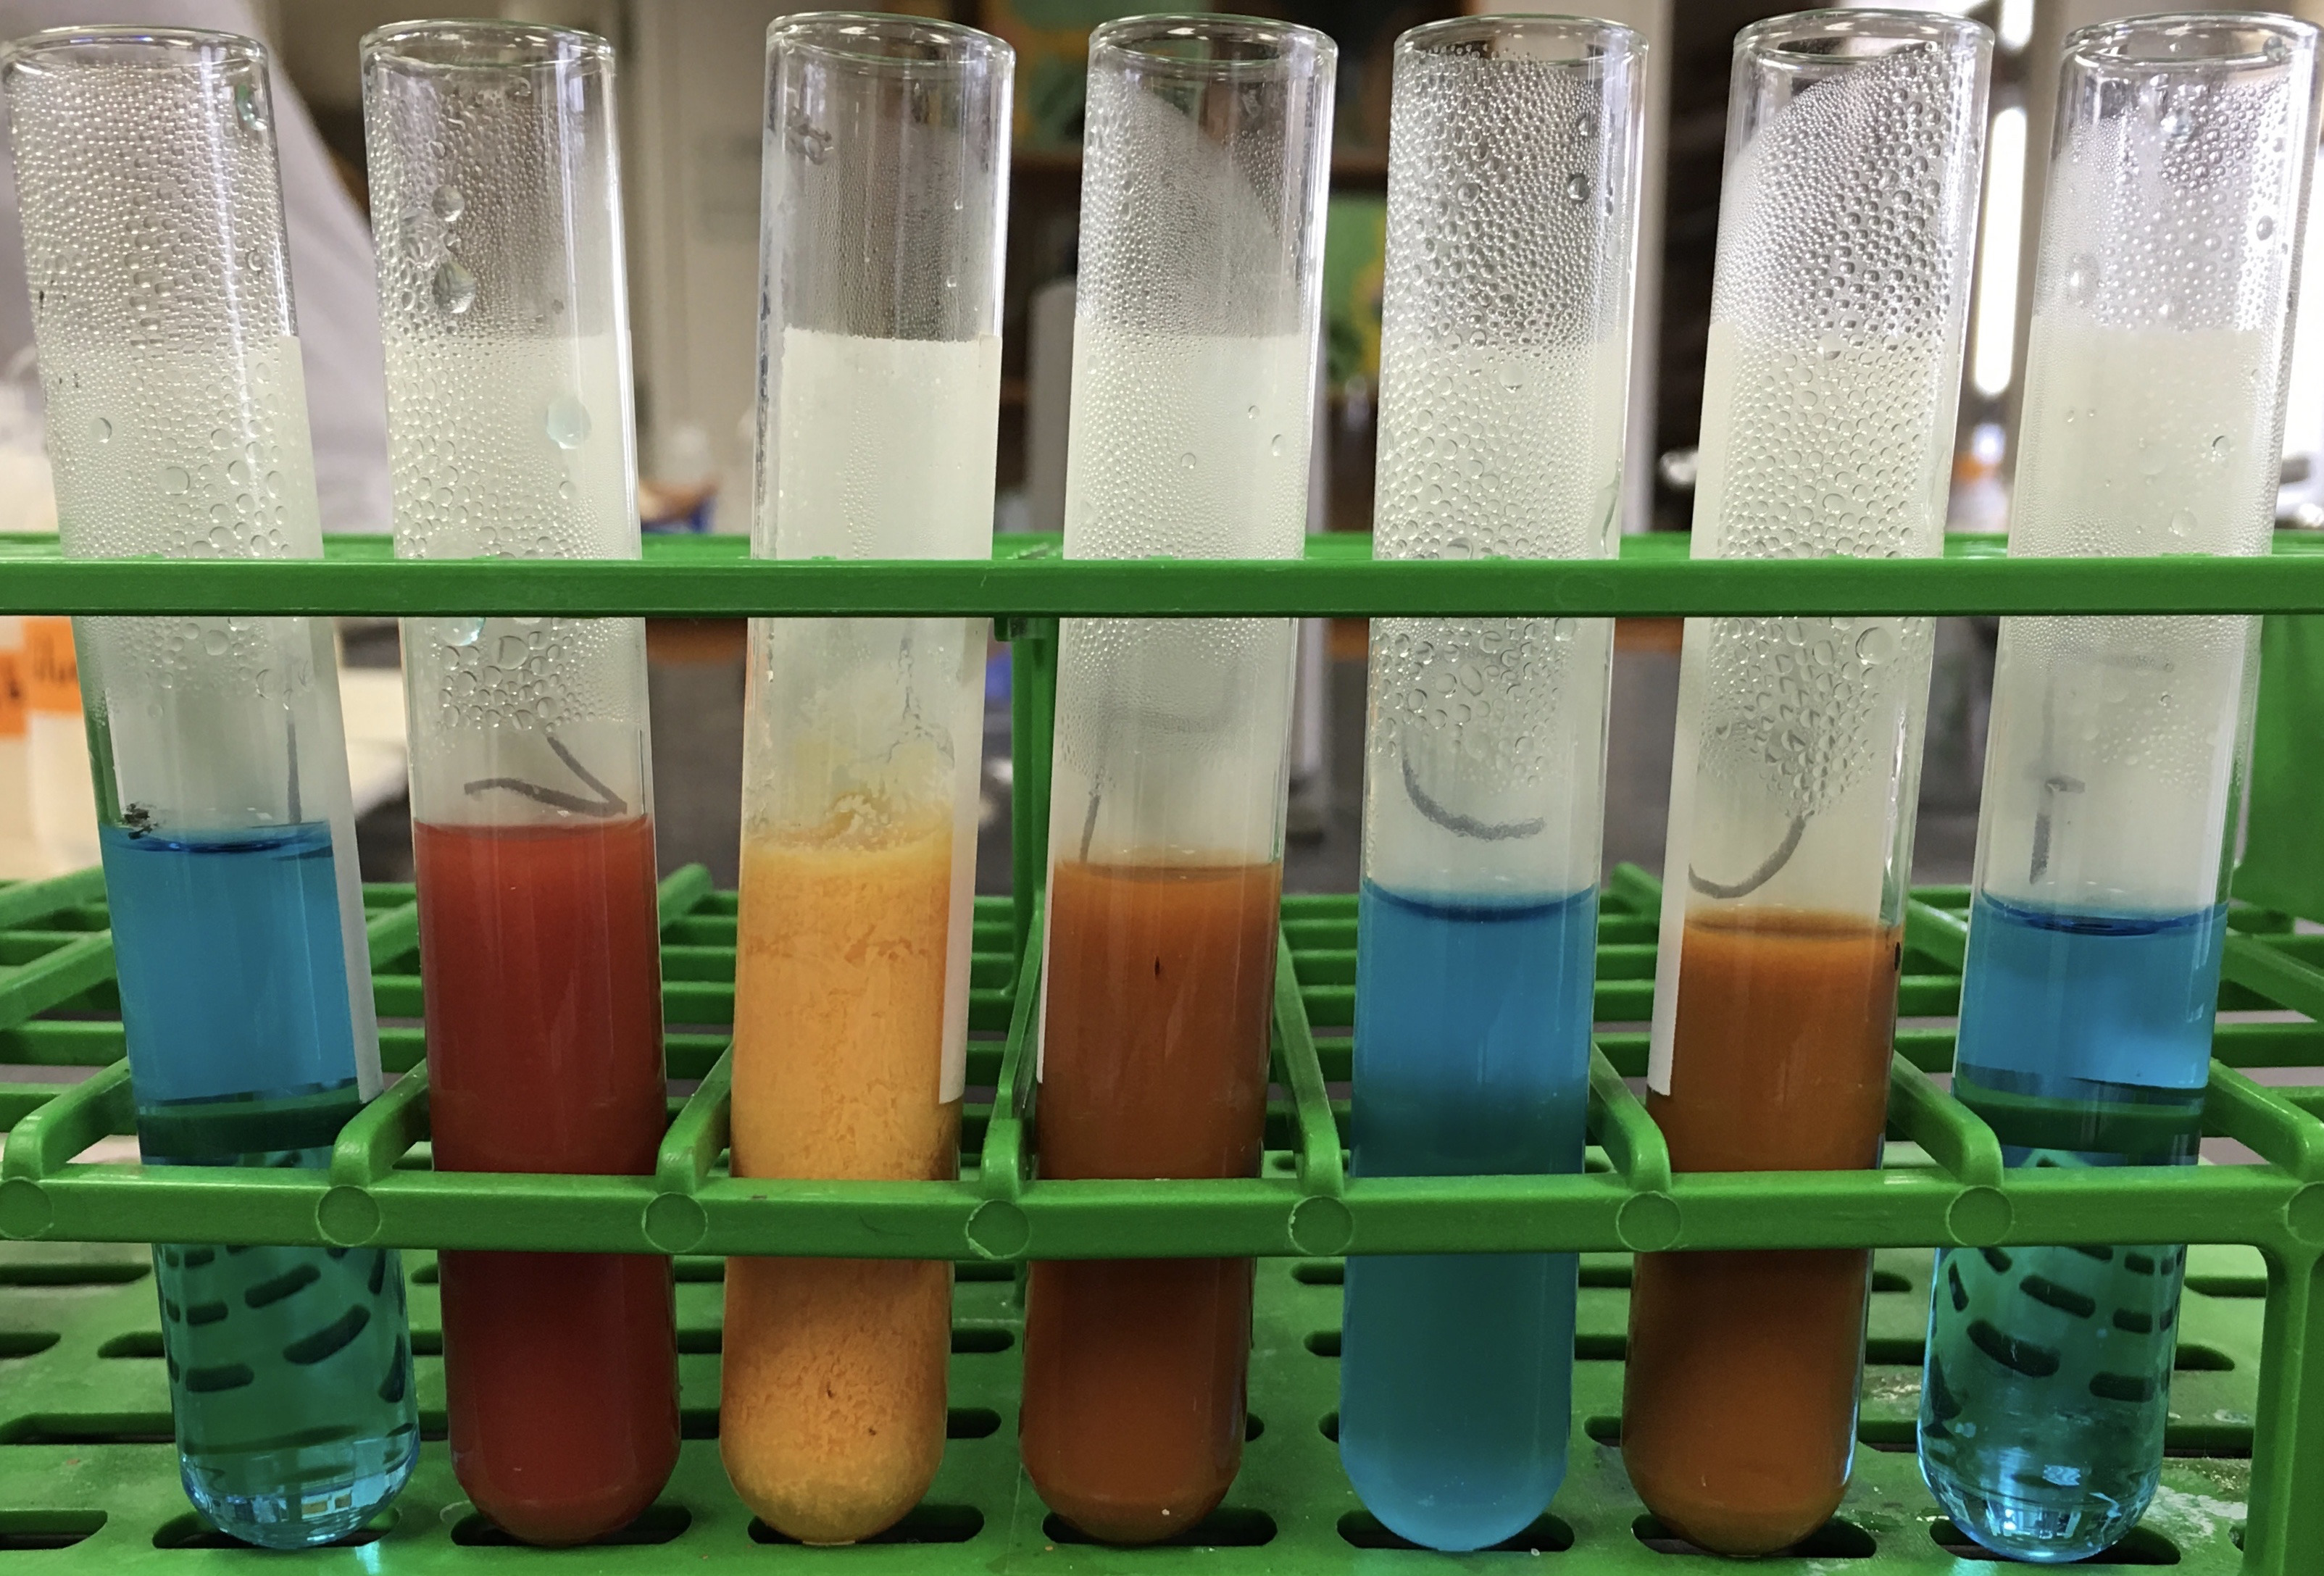
\includegraphics[width=0.7\linewidth]{./figures/chem_aspects/Results_exp_1}

}

\caption{Results from experiment 1. Compare to your results!}\label{fig:exp1}
\end{figure}

\section{Test for Starch}\label{test-for-starch}

Starch is a polymeric carbohydrate consisting of a large number of
glucose units joined by glycosidic bonds. This polysaccharide is
produced by most green plants as energy storage. It is the most common
carbohydrate in human diets and is contained in large amounts in staple
foods like potatoes, wheat, maize (corn), rice, and cassava. Pure starch
is a white, tasteless and odorless powder that is insoluble in cold
water or alcohol. It consists of two types of molecules the linear and
helical amylose and the branched amylopectin.

An \href{https://en.wikipedia.org/wiki/Amylase}{amylase} is an enzyme
that catalyzes the hydrolysis of starch into maltose and glucose.
Amylase is present in the saliva of humans, where it begins the chemical
process of digestion. It is also produced by the pancreas.

\subsection{Experimental procedures}\label{experimental-procedures-2}

\begin{enumerate}
\def\labelenumi{\arabic{enumi}.}
\tightlist
\item
  Obtain 9 plastic test tubes and a test tube rack.
\item
  Using a wax pencil,label each tube with a number (1 to 9).
\item
  Place the tubes from left (tube \#1) to right (tube \#9) in the first
  row of a test tube rack.
\item
  Add the test material to tubes 1 to 9 as indicated in the table below.
  Leave tube 9 empty.
\item
  Check the that the temperature of the heat block is
  \textasciitilde{}37°C and then place tube \#8 in the heat block. Set a
  timer and incubate the tubes for 15 minutes.
\item
  Add 5 drops of Iodine solution to the test tubes \#1 to \# 7. Mix
  well.
\item
  Record the color (in your own words) in in Table \ref{tab:starch}.
\item
  After 15 minutes, remove test tube 8 from the heat block and transfer
  2 ml (half of the contents of test tube 8) to tube 9.
\item
  Add 5 drops of iodine to tube 8 and record your observation in Table
  \ref{tab:starch}.
\item
  Add 2 ml of Benedict's solution to tube \#9.
\item
  Place tube 9 in the \textasciitilde{}65°C heat block. Set a timer and
  incubate the tube for 15 minutes.
\item
  After 15 minutes, remove tube 9 using a test tube holder (be careful,
  it is hot!), place it in the tube rack and record the color (in your
  own words) in the table.
\end{enumerate}

\begin{longtable}[]{@{}clccc@{}}
\caption{\label{tab:starch} Test for starch.}\tabularnewline
\toprule
Tube \# & Test material & Iodine & Observed color & Test Result (+ or
-)\tabularnewline
\midrule
\endfirsthead
\toprule
Tube \# & Test material & Iodine & Observed color & Test Result (+ or
-)\tabularnewline
\midrule
\endhead
1 & 2 ml starch & 5 drops & &\tabularnewline
2 & 2 ml glucose & 5 drops & &\tabularnewline
3 & 2 ml H\textsubscript{2}O & 5 drops & &\tabularnewline
4 & 2 ml sucrose & 5 drops & &\tabularnewline
5 & cotton (cellulose) & 5 drops & &\tabularnewline
6 & a small piece of bread & 5 drops & &\tabularnewline
7 & a small piece of potato & 5 drops & &\tabularnewline
8 & 2 ml of starch plus 2 ml of amylase & 5 drops & &\tabularnewline
9 & Leave empty then follow step 8 above & 2 ml of Benedict's solution &
&\tabularnewline
\bottomrule
\end{longtable}

\begin{figure}

{\centering 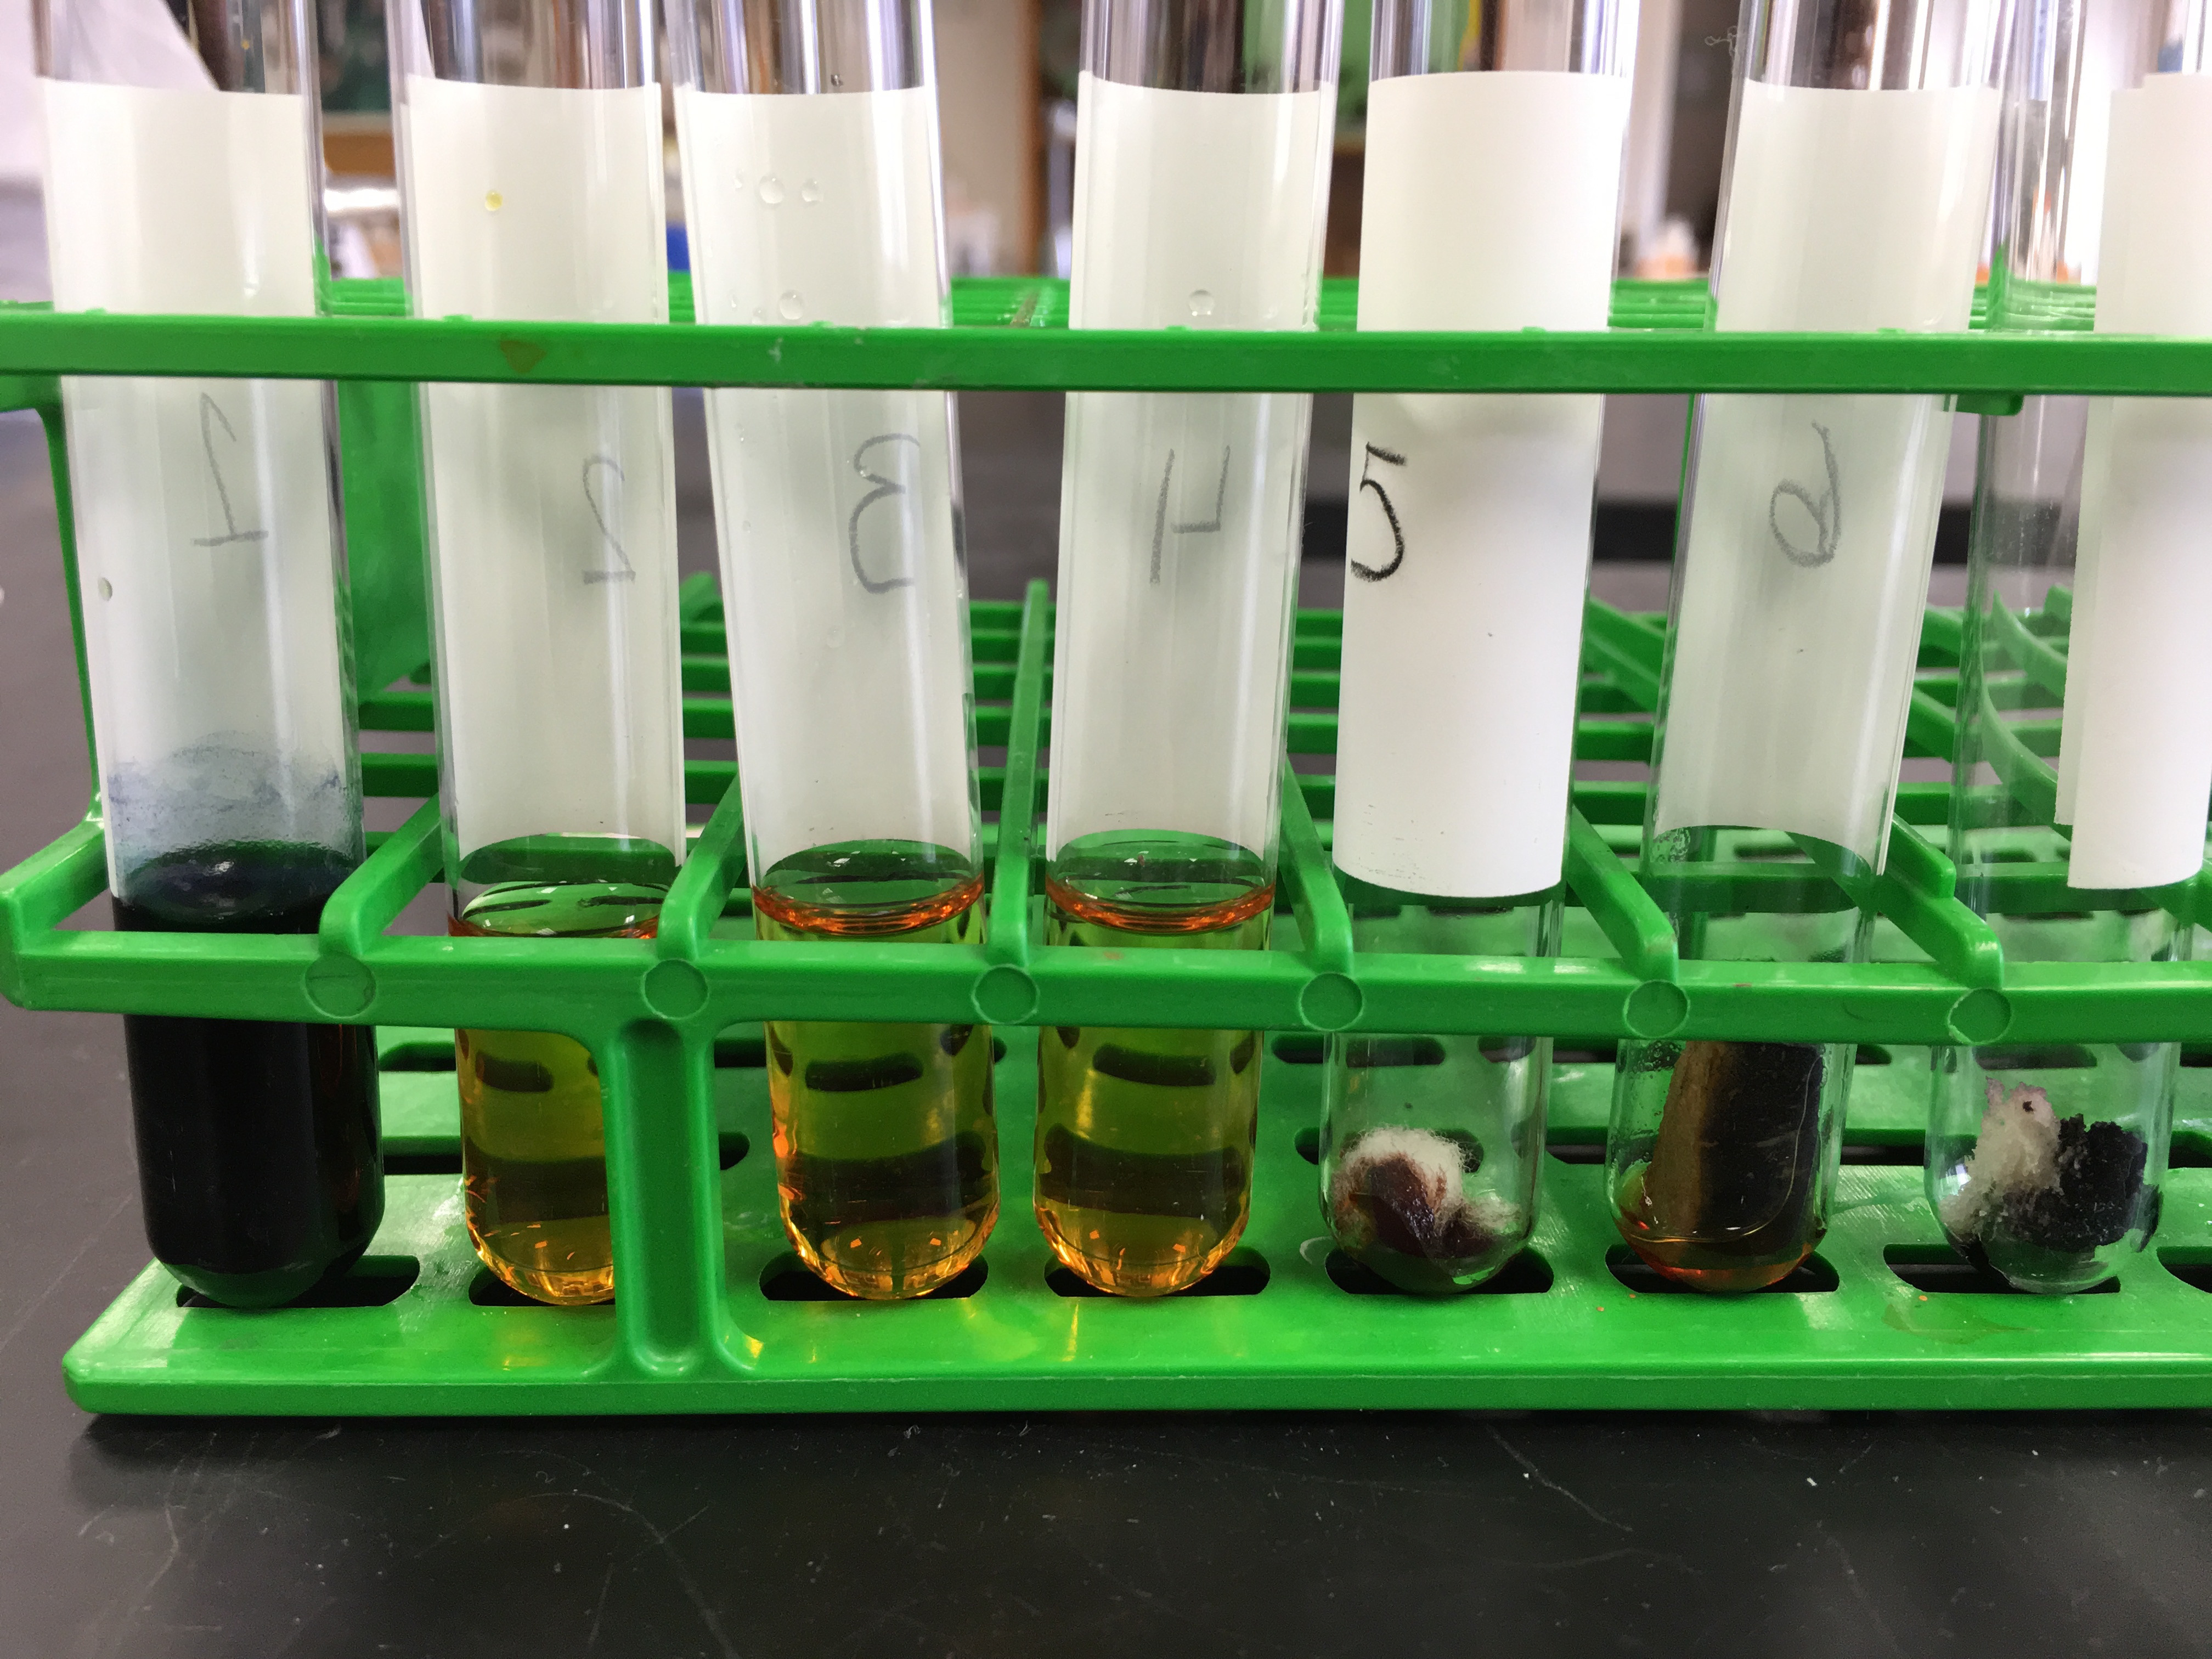
\includegraphics[width=0.7\linewidth]{./figures/chem_aspects/Results_exp_2}

}

\caption{Results from experiment 2. Compare to your results!}\label{fig:exp2}
\end{figure}

\section{Test for Proteins}\label{test-for-proteins}

\href{https://en.wikipedia.org/wiki/Protein}{Proteins} are large
biomolecules, or macromolecules, consisting of one or more long chains
of amino acid residues. Proteins perform a vast array of functions
within organisms, including catalyzing metabolic reactions, DNA
replication, responding to stimuli, and transporting molecules from one
location to another. Proteins differ from one another primarily in their
sequence of amino acids, which is dictated by the nucleotide sequence of
their genes, and which usually results in protein folding into a
specific three-dimensional structure that determines its activity. A
linear chain of amino acid residues is called a polypeptide. A protein
contains at least one long polypeptide. Short polypeptides, containing
less than 20-30 residues, are rarely considered to be proteins and are
commonly called peptides, or sometimes oligopeptides. The individual
amino acid residues are bonded together by peptide bonds and adjacent
amino acid residues. The sequence of amino acid residues in a protein is
defined by the sequence of a gene, which is encoded in the genetic code.
In general, the genetic code specifies 20 standard amino acids; however,
in certain organisms the genetic code can include selenocysteine and-in
certain archaea-pyrrolysine.

The biuret test is a chemical test used for detecting the presence of
peptide bonds. In the presence of peptides, a copper(II) ion forms
violet-colored coordination complexes in an alkaline solution. The
biuret reaction can be used to assess the concentration of proteins
because peptide bonds occur with the same frequency per amino acid in
the peptide. The intensity of the color is directly proportional to the
protein concentration. Despite its name, the reagent does not in fact
contain biuret ((H\textsubscript{2}N-CO-)\textsubscript{2}NH). The test
is named so because it also gives a positive reaction to the
peptide-like bonds in the biuret molecule. In this assay, the copper(II)
binds with nitrogen present in the peptides of proteins. In a secondary
reaction, the copper(II) is reduced to copper(I). Due to its
insensitivity and little interference by free amino acids, this assay is
most useful for whole tissue samples and other sources with high protein
concentration.

\subsection{Experimental procedures}\label{experimental-procedures-3}

\begin{enumerate}
\def\labelenumi{\arabic{enumi}.}
\tightlist
\item
  Obtain 7 plastic test tubes and a test tube rack.
\item
  Using a wax pencil,label each tube with a number (1 to 7).
\item
  Place the tubes from left (tube \#1) to right (tube \#7) in the first
  row of a test tube rack.
\item
  Add the materials to these tubes as indicated in Table
  \ref{tab:protein} and mix well. No heating is needed to produce a
  reaction.
\item
  Wait 2 minutes and then record your observations in the table below.
  Base your conclusion only on the presence or absence of the violet
  color.
\end{enumerate}

\begin{longtable}[]{@{}clccc@{}}
\caption{\label{tab:protein} Test for protein.}\tabularnewline
\toprule
Tube \# & Test material & Biuret & Observation & Test\tabularnewline
\midrule
\endfirsthead
\toprule
Tube \# & Test material & Biuret & Observation & Test\tabularnewline
\midrule
\endhead
1 & 2 ml H\textsubscript{2}O & 2 ml & &\tabularnewline
2 & 2 ml sucrose & 2 ml & &\tabularnewline
3 & 2 ml albumin & 2 ml & &\tabularnewline
4 & 2 ml milk & 2 ml & &\tabularnewline
5 & a small piece of bread & 2 ml & &\tabularnewline
6 & 2 ml soy & 2 ml & &\tabularnewline
7 & 2 ml vegetable oil & 2 ml & &\tabularnewline
\bottomrule
\end{longtable}

\begin{figure}

{\centering 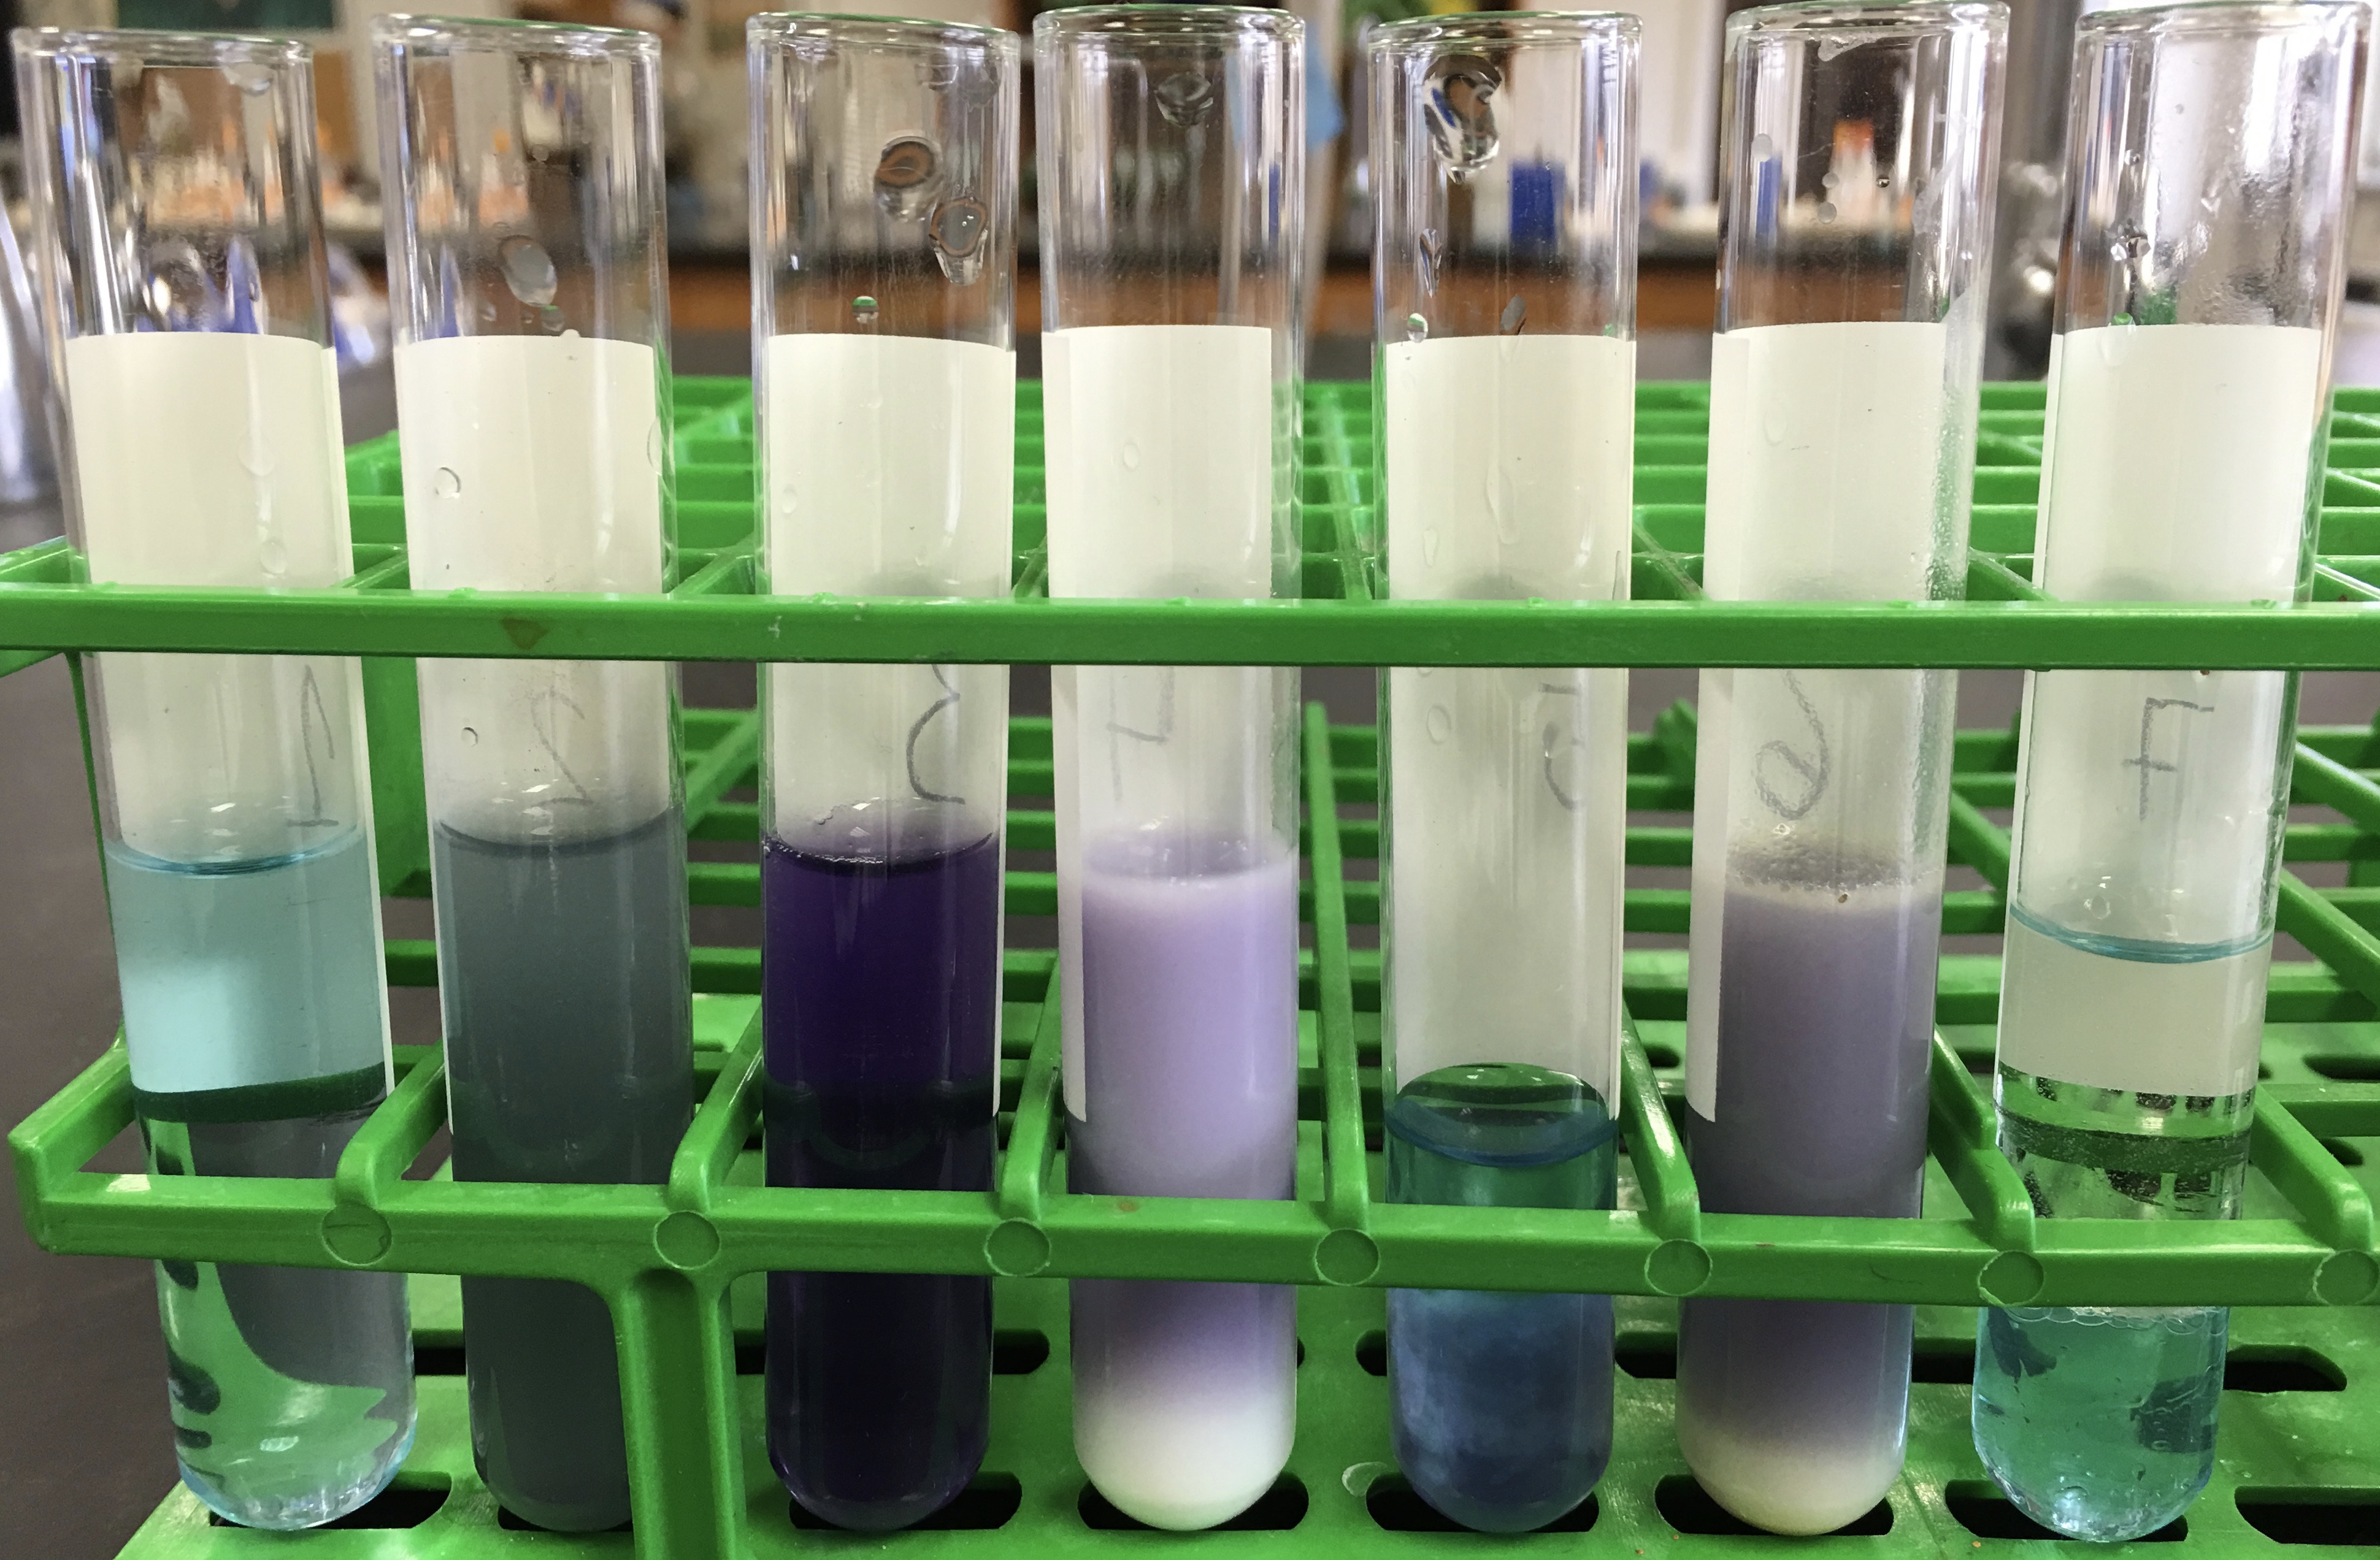
\includegraphics[width=0.7\linewidth]{./figures/chem_aspects/Results_exp_3}

}

\caption{Results from experiment 3. Compare to your results!}\label{fig:exp3}
\end{figure}

\section{Cleaning up}\label{cleaning-up}

\begin{enumerate}
\def\labelenumi{\arabic{enumi}.}
\tightlist
\item
  Empty the contents of all plastic tubes into the labeled waste
  container (brown bottle) in the chemical fume hood.
\item
  Discard the empty tubes in the regular waste basket.
\end{enumerate}

\section{Test for Lipids}\label{test-for-lipids}

In biology, a \href{https://en.wikipedia.org/wiki/Lipid}{lipid} is a
substance of biological origin that is soluble in nonpolar solvents. It
comprises a group of naturally occurring molecules that include fats,
waxes, sterols, fat-soluble vitamins (such as vitamins A, D, E, and K),
monoglycerides, diglycerides, triglycerides, and phospholipids. The main
biological functions of lipids include storing energy, signaling, and
acting as structural components of cell membranes. Lipids have
applications in the cosmetic and food industries as well as in
nanotechnology. Scientists sometimes broadly define lipids as
hydrophobic or amphiphilic small molecules; the amphiphilic nature of
some lipids allows them to form structures such as vesicles, liposomes,
or membranes in an aqueous environment. Although the term ``lipid'' is
sometimes used as a synonym for fats, fats are a subgroup of lipids
called triglycerides. Lipids also encompass molecules such as fatty
acids and their derivatives (including tri-, di-, mono-glycerides, and
phospholipids), as well as other sterol-containing metabolites such as
cholesterol. Although humans and other mammals use various biosynthetic
pathways both to break down and to synthesize lipids, some essential
lipids cannot be made this way and must be obtained from the diet.

\subsection{Experimental procedures}\label{experimental-procedures-4}

\begin{enumerate}
\def\labelenumi{\arabic{enumi}.}
\tightlist
\item
  Obtain a small glass tube.
\item
  Add 2 ml of water into the glass tube.
\item
  Add 6 drops of vegetable oil to on top.
\item
  Shake thoroughly and observe the way the oil is dispersed only
  temporarily. This is an emulsion a mixture of two liquids, each
  insoluble in the other.
\item
  Now add 3 drops of lipid-specific red Sudan stain and mix again.
\item
  Add 2 ml of a liquid detergent to the tube and shake again.
\item
  Allow the tube to stand and note that the two phases (oil and water)
  are no longer distinctly separated. Detergent is often termed an
  emulsifier. Its molecules are water-soluble on one end and
  lipid-soluble on the other. These surround small oil droplets,
  water-soluble end out, and allow the droplets to stay suspended in the
  water.
\end{enumerate}

\section{Cleaning up}\label{cleaning-up-1}

Empty the contents of the glass tube into the labeled waste container
(brown bottle) in the chemical fume hood. Discard the glass tube in the
plastic container labeled ``broken glass'' in the chemical fume hood.

\section{Test for organic and inorganic compounds
(Demonstration)}\label{test-for-organic-and-inorganic-compounds-demonstration}

\subsection{Experimental procedures}\label{experimental-procedures-5}

\begin{enumerate}
\def\labelenumi{\arabic{enumi}.}
\tightlist
\item
  The instructor will use as Bunsen burner to heat a number of
  substances. Organic substances will burn, inorganic substances will
  remain unchanged.
\item
  Record your observation in Table \ref{tab:organic}.
\end{enumerate}

\begin{longtable}[]{@{}lcc@{}}
\caption{\label{tab:organic} Test for organic and inorganic
compounds.}\tabularnewline
\toprule
Substance & Organic & Inorganic\tabularnewline
\midrule
\endfirsthead
\toprule
Substance & Organic & Inorganic\tabularnewline
\midrule
\endhead
sugar & &\tabularnewline
table salt & &\tabularnewline
baking soda & &\tabularnewline
unknown & &\tabularnewline
\bottomrule
\end{longtable}

\section{Strawberry DNA extraction}\label{strawberry-dna-extraction}

We will use strawberries for
\href{https://en.wikipedia.org/wiki/DNA}{DNA} isolation. Wild
strawberries (Fragaria vesca) are ``diploid'' organisms (two sets of
chromosomes; 14 total), just like us, but the at a size of 240 million
base the strawberry genome (which has been fully sequenced) is much
smaller than ours (3 billion bases). The cultivated strawberry, Fragaria
ananassa, were generated only about 250 years ago are thus a very young
crop species. Botanically, it is neither a berry nor a true fruit.
Strawberry ``fruits'' consist of dry seeds that dot the surface of a
fleshy modified shoot tip (the receptacle). Genomically, Fragaria
ananassa is among the most complex of crop plants they harbor eight sets
of chromosomes (2n = 8× = 56), which are originally derived from as many
as four different diploid ancestors. Thus, \emph{Fragaria ananassa}, is
an octoploid organism, with 4 times more DNA in each cell than wild
strawberries. This property makes this fruit a great choice for
demonstrating DNA extraction. In addition, strawberries are soft and
easy to homogenize and ripe.

The first step of DNA extraction from live or dead cells is to lyse or
break open the cell. After the cells have broken open, a salt solution
such as sodium chloride (NaCl) and a detergent solution containing the
compound SDS (sodium dodecyl sulfate) is added. This solution breaks
down and emulsifies the fat \& proteins that make up the cell membrane.
Finally, ice cold ethanol is added. The alcohol and salt cause the DNA
to precipitate, or settle out of the solution, leaving behind all the
cellular components that aren't soluble in alcohol. The DNA can be
spooled (wound) on a stirring rod and pulled from the solution at this
point.

It is important to mention that the procedure for DNA extraction we are
using is really a procedure for total nucleic acid extraction. However,
much of the RNA extracted is cut by ribonucleases (enzymes that cut RNA)
that come in contact with the RNA when the cells are broken open.

\subsection{Experimental procedures}\label{experimental-procedures-6}

\begin{enumerate}
\def\labelenumi{\arabic{enumi}.}
\tightlist
\item
  Place 2 to 4 strawberries in a zip lock bag. Gently, mash up the fruit
  by pushing the bags with your hand against the lab bench. This will
  mechanically breakdown the cell wall.
\item
  Add 15 ml of the extraction buffer to the bag. Mix and mash again for
  one minute (chemical portion of the extraction procedure to lyse the
  cell membranes to release the DNA).
\item
  Filter the homogenate using cheesecloth. Hold the cheesecloth over the
  beaker with the help of a rubber band. This step removes cell
  organelles, broken cell walls, membrane fragments, and other cell
  debris.
\item
  Collect the filtrate; squeeze the cheesecloth to get the as much of
  the lysate as possible.
\item
  Pour the filtrate into a plastic tube. Fill the tube to about half the
  volume
\item
  Use the transfer pipet to drip alcohol slowly down the sides of the
  tube (about 5 ml of ice cold alcohol), while holding the tube at
  approximately an angle of 45o. Try to make a clear and undisturbed
  layer of alcohol to float on the lysate. The line between the two
  layers is called the interface.
\item
  At the interface, you will see the DNA precipitate out of solution and
  float to the top. Spool the DNA on your glass rod.
\end{enumerate}

\section{Cleaning up}\label{cleaning-up-2}

\begin{enumerate}
\def\labelenumi{\arabic{enumi}.}
\tightlist
\item
  Empty the contents of the plastic tube into the labeled waste
  container (brown bottle) in the chemical fume hood.
\item
  Discard the empty tubes and other waste in the regular waste basket.
\item
  Rinse the glass rod and glassware with water and detergent.
\item
  Return the glass rod and glass ware to the trays on your bench where
  you originally found them.
\end{enumerate}

\section{Review Questions}\label{review-questions-1}

\begin{enumerate}
\def\labelenumi{\arabic{enumi}.}
\tightlist
\item
  What are organic compounds?
\item
  Which are the five most common elements in living organisms?
\item
  What are the four major groups of biomacromolecules?
\item
  What are the building blocks (monomers) of DNA?
\item
  What are lipids?
\item
  What are proteins?
\item
  What is a peptide bond?
\item
  What is chemical reduction?
\item
  What is chemical oxidation?
\item
  What are detergents?
\item
  Why do we use the detergent in the DNA extraction experiment?
\end{enumerate}
